
En esta sección se presentan los resultados obtenidos a partir de la ejecución de los programas desarrollados. 
Estos resultados se representan en gráficas que permiten visualizar y analizar el comportamiento de los algoritmos implementados.
Antes de analizar los algoritmos de ordenamiento, se muestra un resumen de las complejidades teoricas del tiempo de ejecucion de los distintos algoritmos.\\
\textbf{Complejidad teórica:}
\begin{itemize}
    \item Merge Sort: O(n log n) peor caso y promedio.
    \item Quick Sort: O($n^2$) peor caso, O(n log n) promedio.
    \item Sort (std::sort): O(n log n) promedio y peor caso.
\end{itemize}

\begin{figure}[H]
    \centering
    \begin{minipage}[t]{0.5\textwidth}
        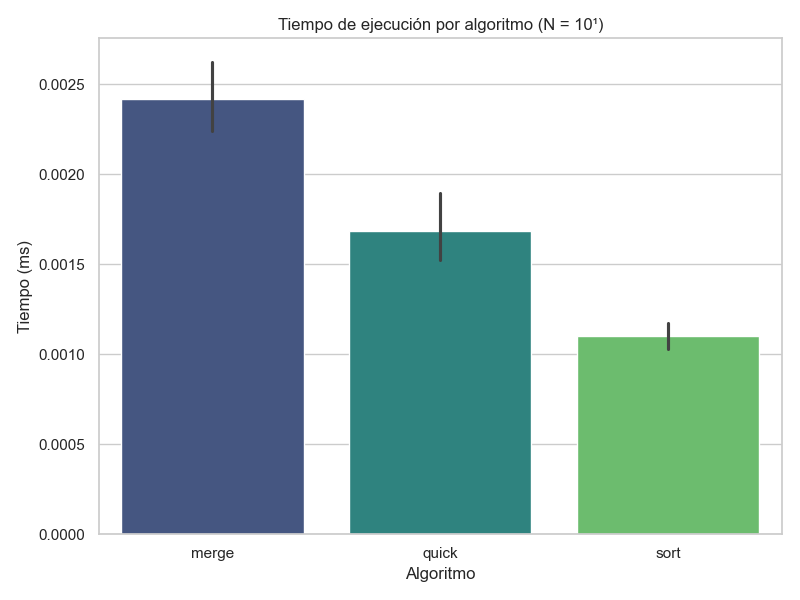
\includegraphics[width=\textwidth]{../code/sorting/data/plots/tiempo_algoritmos_N10_barra.png}
    \end{minipage}%
    \caption{N = 10}
    \label{fig:scatterplot_3}
\end{figure}

\begin{figure}[H]
    \centering
    \begin{minipage}[t]{0.5\textwidth}
        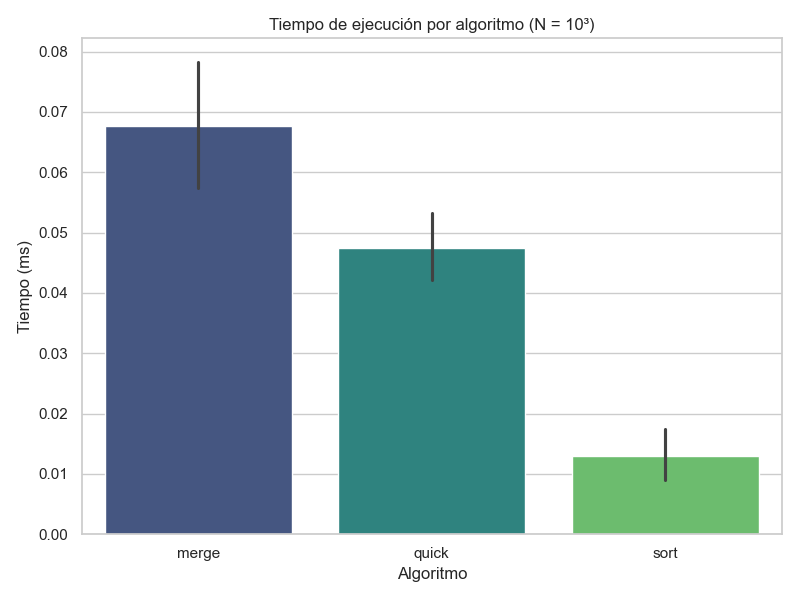
\includegraphics[width=\textwidth]{../code/sorting/data/plots/tiempo_algoritmos_N100_barra.png}
    \end{minipage}%
    \caption{N = 1000}
    \label{fig:scatterplot_3}
\end{figure}

\begin{figure}[H]
    \centering
    \begin{minipage}[t]{0.5\textwidth}
        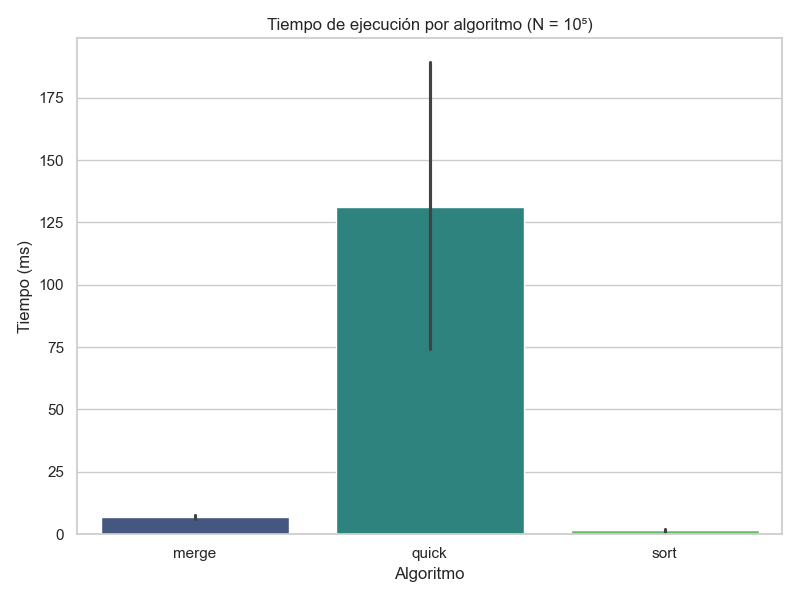
\includegraphics[width=\textwidth]{../code/sorting/data/plots/tiempo_algoritmos_N100000_barra.png}
    \end{minipage}%
    \caption{N = 100000}
    \label{fig:scatterplot_3}
\end{figure}

\textbf{Análisis de tiempos por tamaño de arreglo (N)} : Fig. 1, 2 y 3.
\begin{itemize}
    \item \textbf{N = 10:} Merge Sort presenta el mayor tiempo de ejecución, mientras que Quick Sort y Sort muestran los menores tiempos. 
    Debido al tamaño reducido del arreglo, todos los algoritmos tienen tiempos muy bajos (máximo $\approx 0.0025$ ms), pero comparándolos se observan diferencias significativas.
    \item \textbf{N = 1.000:} Al analizar con un aumento de N, podemos notar que sigue la misma tendencia que con $N = 10$, pero con tiempos mas elevados (alrededor de $\approx 0.07$ ms para Merge Sort). Además se observa que Sort destaca con un tiempo pequeño ($\approx 0.01$ ms).
    \item \textbf{N = 100.000:} Quick Sort es el que tiene el tiempo de ejecución más elevado ($\approx 125$ ms, con alta variabilidad), mientras que Merge Sort y Sort tienen tiempos menores a 5 ms y cercanos a 0. Esto se explica por la dependencia de Quick Sort respecto a la elección del pivote, lo que puede degradar su rendimiento en ciertos casos.
\end{itemize}

\begin{figure}[H]
    \centering
    \begin{minipage}[t]{0.5\textwidth}
        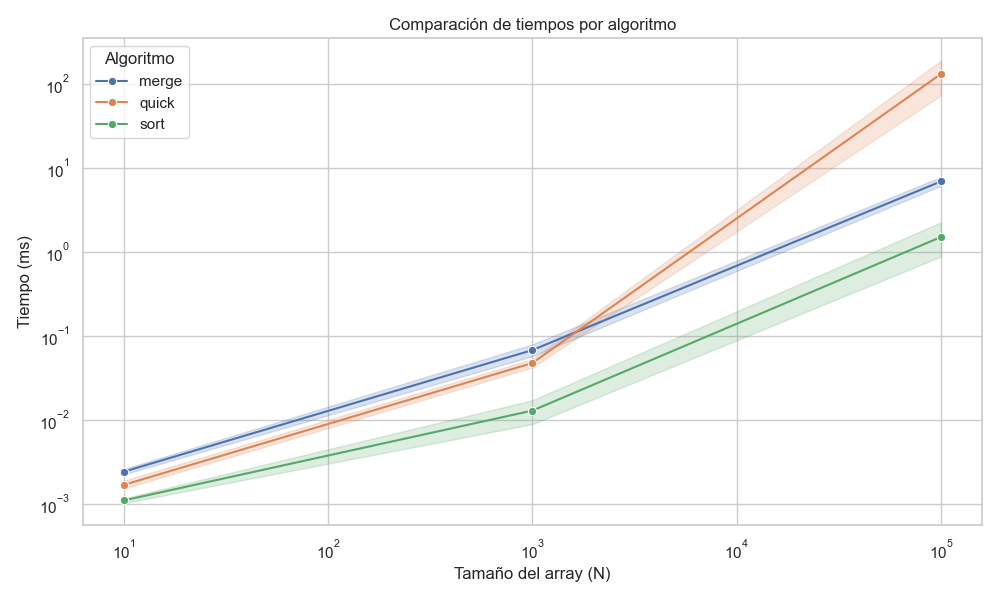
\includegraphics[width=\textwidth]{../code/sorting/data/plots/tiempos_algoritmos.png}
    \end{minipage}%
    \caption{Tiempo por algoritmo}
    \label{fig:scatterplot_3}
\end{figure}


\textbf{Análisis de crecimiento de tiempo vs tamaño (N)} : Fig. 4.

Se observa claramente cómo los tiempos de ejecución aumentan con el tamaño del arreglo. 
Merge Sort y Sort presentan una tendencia de crecimiento similar (\textbf{O(n log n)}), siendo Sort el más eficiente de los dos, lo cual refleja optimizaciones adicionales.
El Quick Sort tiene un aumento en el tiempo de ejecución en arreglos mayores de $10^5$ principalmente por el pivote.
\begin{figure}[H]
    \centering
    \begin{minipage}[t]{0.5\textwidth}
        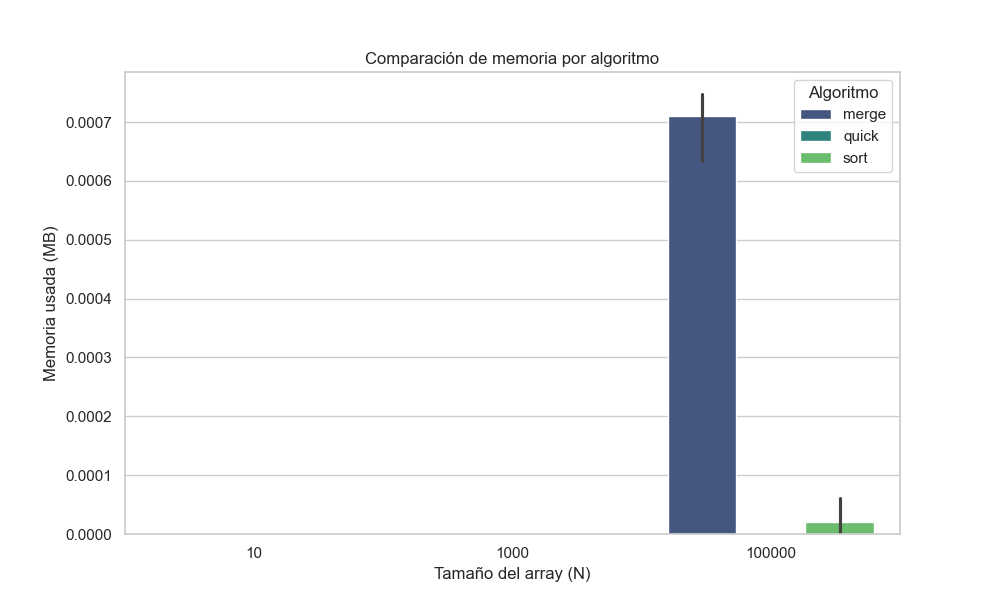
\includegraphics[width=\textwidth]{../code/sorting/data/plots/memoria_algoritmos_barras.png}
    \end{minipage}%
    \caption{Memoria por algoritmo}
    \label{fig:scatterplot_3}
\end{figure}

\textbf{Análisis de memoria vs tamaño (N)} : Fig. 5.

\begin{itemize}
\item Arreglos de tamaño 10 y 1.000: Todos los algoritmos ocupan aproximadamente la misma memoria, debido a la el tamaño pequeño de los arreglos de cada implementación.

\item Arreglos de tamaño 100.000: Merge Sort utiliza una gran cantidad de memoria en comparación con los otros algoritmos. Sort ocupa memoria cercana al 0, mientras que Quick Sort no ocupa memoria extra.
\end{itemize}

\begin{figure}[H]
    \centering
    \begin{minipage}[t]{0.5\textwidth}
        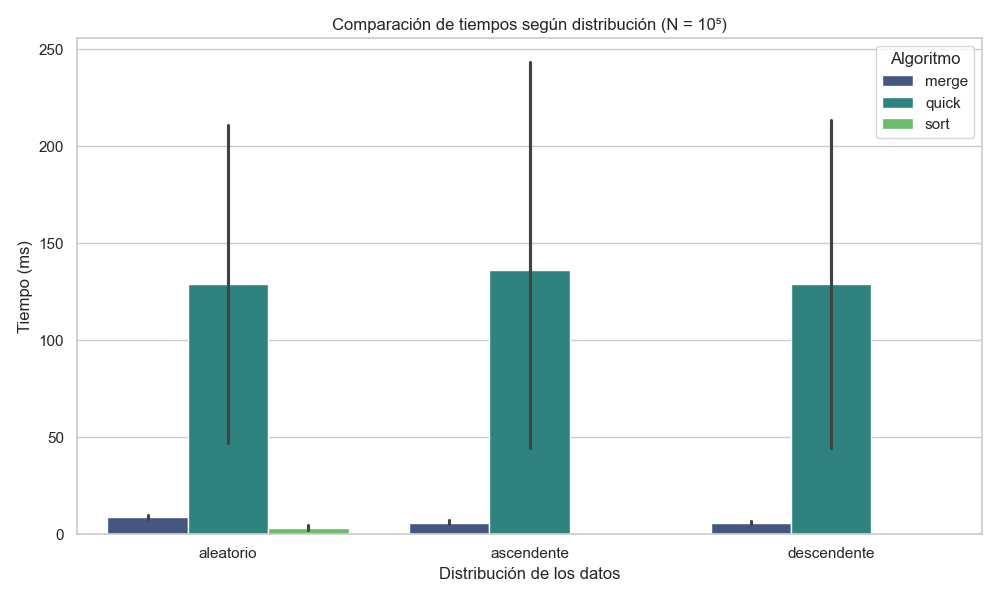
\includegraphics[width=\textwidth]{../code/sorting/data/plots/tiempo_por_distribucion.png}
    \end{minipage}%
    \caption{Memoria por algoritmo}
    \label{fig:scatterplot_3}
\end{figure}

\textbf{Análisis de tiempo vs distribución (Aleatoria, ascendente y descendente)} : Fig. 6.
Al analizar como afecta la distribución se puede apreciar que para los algoritmos Sort y Merge sort no hay mucha diferencia en los tiempos. También se mantiene esto en Quick Sort pero con una varianza en todas las distribuciones, por
lo que es relativo el tiempo que toma en ordenar el arreglo.

\textbf{Antes de analizar los algoritmos de multiplicacion, se muestra un resumen de las complejidades teoricas del tiempo de ejecucion de los distintos algoritmos.}

\textbf{Marco teórico:}  
\begin{itemize}
    \item \textbf{Naive:} complejidad temporal de $O(n^3)$, derivada de los tres bucles anidados que recorren filas y columnas.
    \item \textbf{Strassen:} reduce la complejidad a aproximadamente $O(n^{2.81})$ mediante la descomposición recursiva y uso de 7 multiplicaciones de submatrices en lugar de 8. 
    Aunque es teóricamente más eficiente, en dimensiones pequeñas la sobrecarga de la recursión provoca que sea más lento que el método clásico.
\end{itemize}

\begin{figure}[H]
    \centering
    \begin{minipage}[t]{0.5\textwidth}
        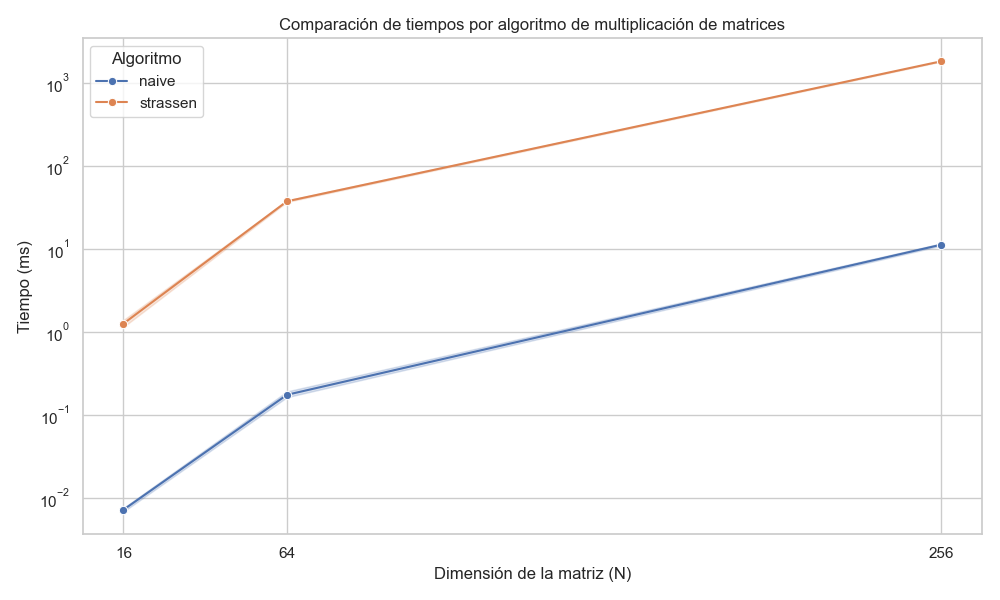
\includegraphics[width=\textwidth]{../code/matrix_multiplication/data/plots/tiempos_matrices.png}
    \end{minipage}%
    \caption{Tiempo por algoritmo}
    \label{fig:scatterplot_3}
\end{figure}

\textbf{Análisis de tiempo (T) vs tamaño de matriz (N)}: Fig. 6.

En la comparación del tiempo de ejecución según la dimensión de la matriz, ambos algoritmos muestran un crecimiento similar, lo cual es consistente con que ambos tienen complejidad superior a lineal. 
No obstante, se observa que el algoritmo \textbf{Naive} comienza con valores de tiempo más bajos que Strassen para dimensiones pequeñas. 
Esto ocurre porque el método de Strassen introduce sobrecarga por la recursión y las operaciones adicionales necesarias para dividir y combinar submatrices.

\begin{figure}[H]
    \centering
    \begin{minipage}[t]{0.5\textwidth}
        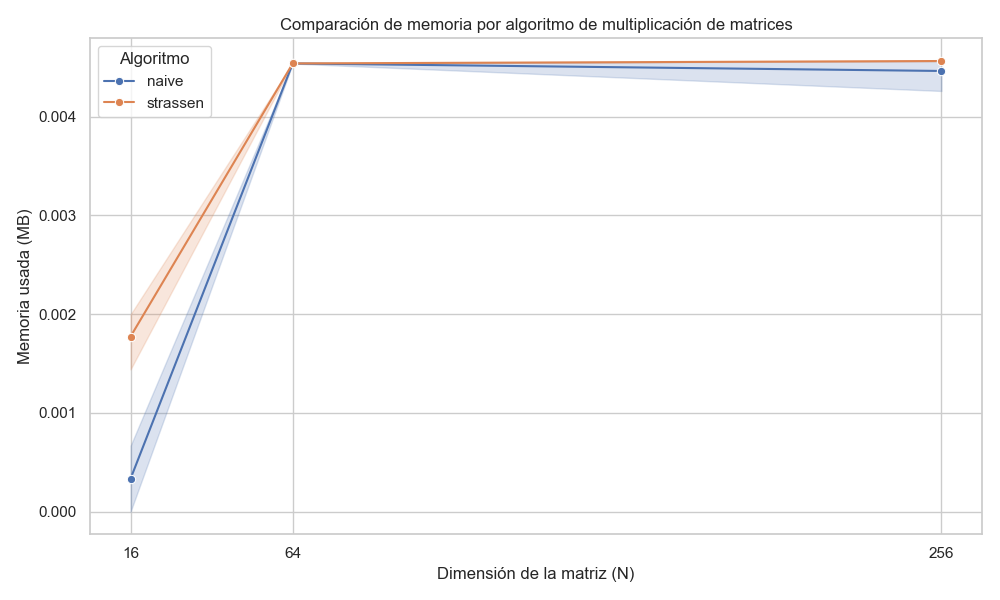
\includegraphics[width=\textwidth]{../code/matrix_multiplication/data/plots/memoria_matrices.png}
    \end{minipage}%
    \caption{Memoria por algoritmo}
    \label{fig:scatterplot_3}
\end{figure}


\textbf{Análisis de uso de memoria vs tamaño de la matriz (N)}

En la comparación de memoria utilizada, se observa un aumento pronunciado al pasar de matrices de dimensión 16 a 64. 
Sin embargo, después de ese punto, el crecimiento se estabiliza, mostrando un patrón más controlado. 
Además, se aprecia que el algoritmo \textbf{Naive} requiere menos memoria que Strassen en todas las dimensiones evaluadas. 
Esto se debe a que Strassen utiliza estructuras adicionales para almacenar submatrices y realizar llamadas recursivas.
 
\begin{itemize}
    \item \textbf{Naive:} el uso de memoria se limita a las matrices de entrada y salida, manteniéndose en $O(n^2)$.
    \item \textbf{Strassen:} requiere espacio adicional para submatrices temporales en cada nivel de recursión, lo que incrementa el uso de memoria hasta $O(n^2 \log n)$ en algunas implementaciones prácticas.
\end{itemize}

\begin{figure}[H]
    \centering
    \begin{minipage}[t]{0.5\textwidth}
        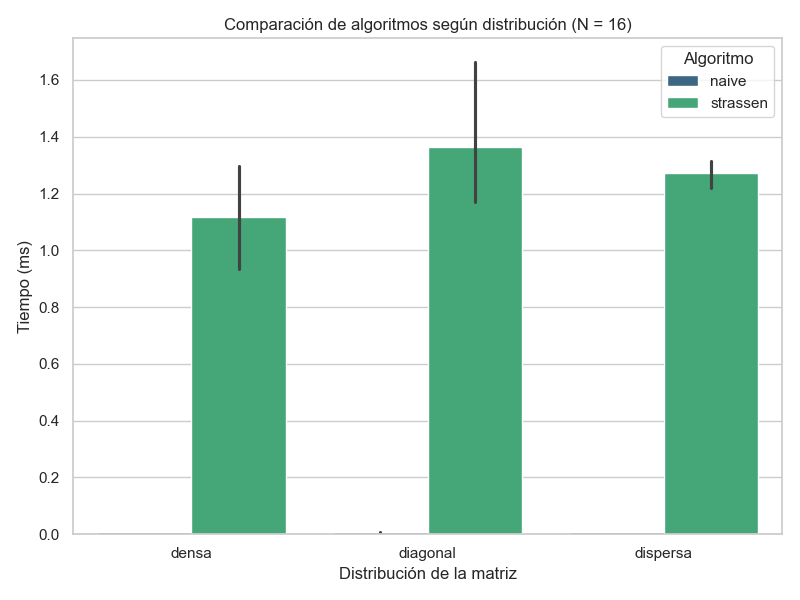
\includegraphics[width=\textwidth]{../code/matrix_multiplication/data/plots/tiempo_matrices_por_distribucion.png}
    \end{minipage}%
    \caption{Tiempo según distribución}
    \label{fig:scatterplot_3}
\end{figure}
Para el algoritmo \textbf{Naive} no existe una diferencia en la distribución pero para \textbf{Strassen} existe una pequeña diferencia de tiempo, siendo la diagonal la más compleja de procesar.

Los resultados muestran que, aunque Strassen es teóricamente más eficiente en tiempo asintótico, para dimensiones pequeñas el algoritmo Naive resulta más rápido y más ligero en memoria. 